\documentclass[/home/jesse/Analysis/FemtoAnalysis/AnalysisNotes/AnalysisNoteJBuxton.tex]{subfiles}
\begin{document}

\subsubsection{\texorpdfstring{$\rm K^{0}_{S}$}{TEXT} Reconstruction}
\label{K0sReconstruction}

The following cuts, in addition to the misidentification and shared daughter cuts presented in Sec. \ref{GenV0Reco}, were used to select good \Ks candidates:

\begin{table}[htbp]
 \centering
%  \renewcommand{\arraystretch}{1.5}
  \begin{tabular}{lc|c|l}
   \hline  
   \multicolumn{4}{c}{\textbf{\Ks reconstruction}} \\
   \hline
   \multicolumn{3}{l|}{$|\eta|$} & $< 0.8$ \\
   \hline
   \multicolumn{3}{l|}{$p_{\mathrm{T}}$} & $> 0.2$ GeV/\textit{c} \\
   \hline
   \multicolumn{4}{l}{$m_{PDG}-13.677 \ \mathrm{MeV} < m_{\mathrm{inv}} < m_{\mathrm{PDG}} + 2.0323 \ \mathrm{MeV}$} \\ 
   \hline
   \multicolumn{3}{l|}{DCA to prim. vertex} & $<$ 0.3 cm \\
   \hline
   \multicolumn{3}{l|}{Cosine of pointing angle} & $>$ 0.9993 \\
   \hline
   \multicolumn{3}{l|}{OnFlyStatus} & false \\
   \hline
   \multicolumn{3}{l|}{Decay Length} & $<$ 30 cm \\
   \hline
   \multicolumn{3}{l|}{Shared Daughter Cut} & true \\
   \hline
   \multicolumn{3}{l|}{Misidentification Cut} & true \\
   \hline   
      
   
   \multicolumn{4}{c}{\textbf{$\pi^{\pm}$ Daughter Cuts}} \\
   \hline
   \multicolumn{3}{l|}{$|\eta|$} &  $< 0.8$ \\
   \hline
   \multicolumn{3}{l|}{Number of clusters in TPC} & $>$ 80 \\
   \hline
   \multicolumn{3}{l|}{Daughter Status} & kTPCrefit \\
   \hline
   \multicolumn{3}{l|}{DCA $\pi^{+}\pi^{-}$ Daughters} & $<$ 0.3 cm \\
   \hline
   \multicolumn{3}{l|}{$p_{\mathrm{T}}$} & $>$ 0.15 GeV/\textit{c} \\
   \hline
   \multicolumn{3}{l|}{DCA to prim vertex} & $>$ 0.3 cm \\
   \hline
   \multicolumn{4}{l}{TPC and TOF N$\sigma$ Cuts} \\
   \hline
    & \multicolumn{1}{c}{$p <$ 0.5 GeV/\textit{c}} &  & N$\sigma_{\mathrm{TPC}} <$ 3 \\
   \hline
    & \multirow{2}{*}{$p >$ 0.5 GeV/\textit{c}} &  if TOF \& TPC available & N$\sigma_{\mathrm{TPC}} <$ 3 \& N$\sigma_{\mathrm{TOF}} <$ 3 \\
   \cline{3-4}
    & & else & N$\sigma_{\mathrm{TOF}} <$ 3 \\
   \hline   
  \end{tabular}
% \end{minipage}
 \caption[\Ks reconstruction]{\Ks reconstruction}
 \label{tab:K0sCuts} 
\end{table}

\begin{figure}[h!]
  \centering
  %%----start of first subfigure---  
  \subfloat[Mass assuming \Lam-hypothesis for \Ks collection, i.e. assume the daughters are $p^{+}\pi^{-}$ instead of $\pi^{+}\pi^{-}$.]{
    \label{fig:MassAsscLamHyp:a}
    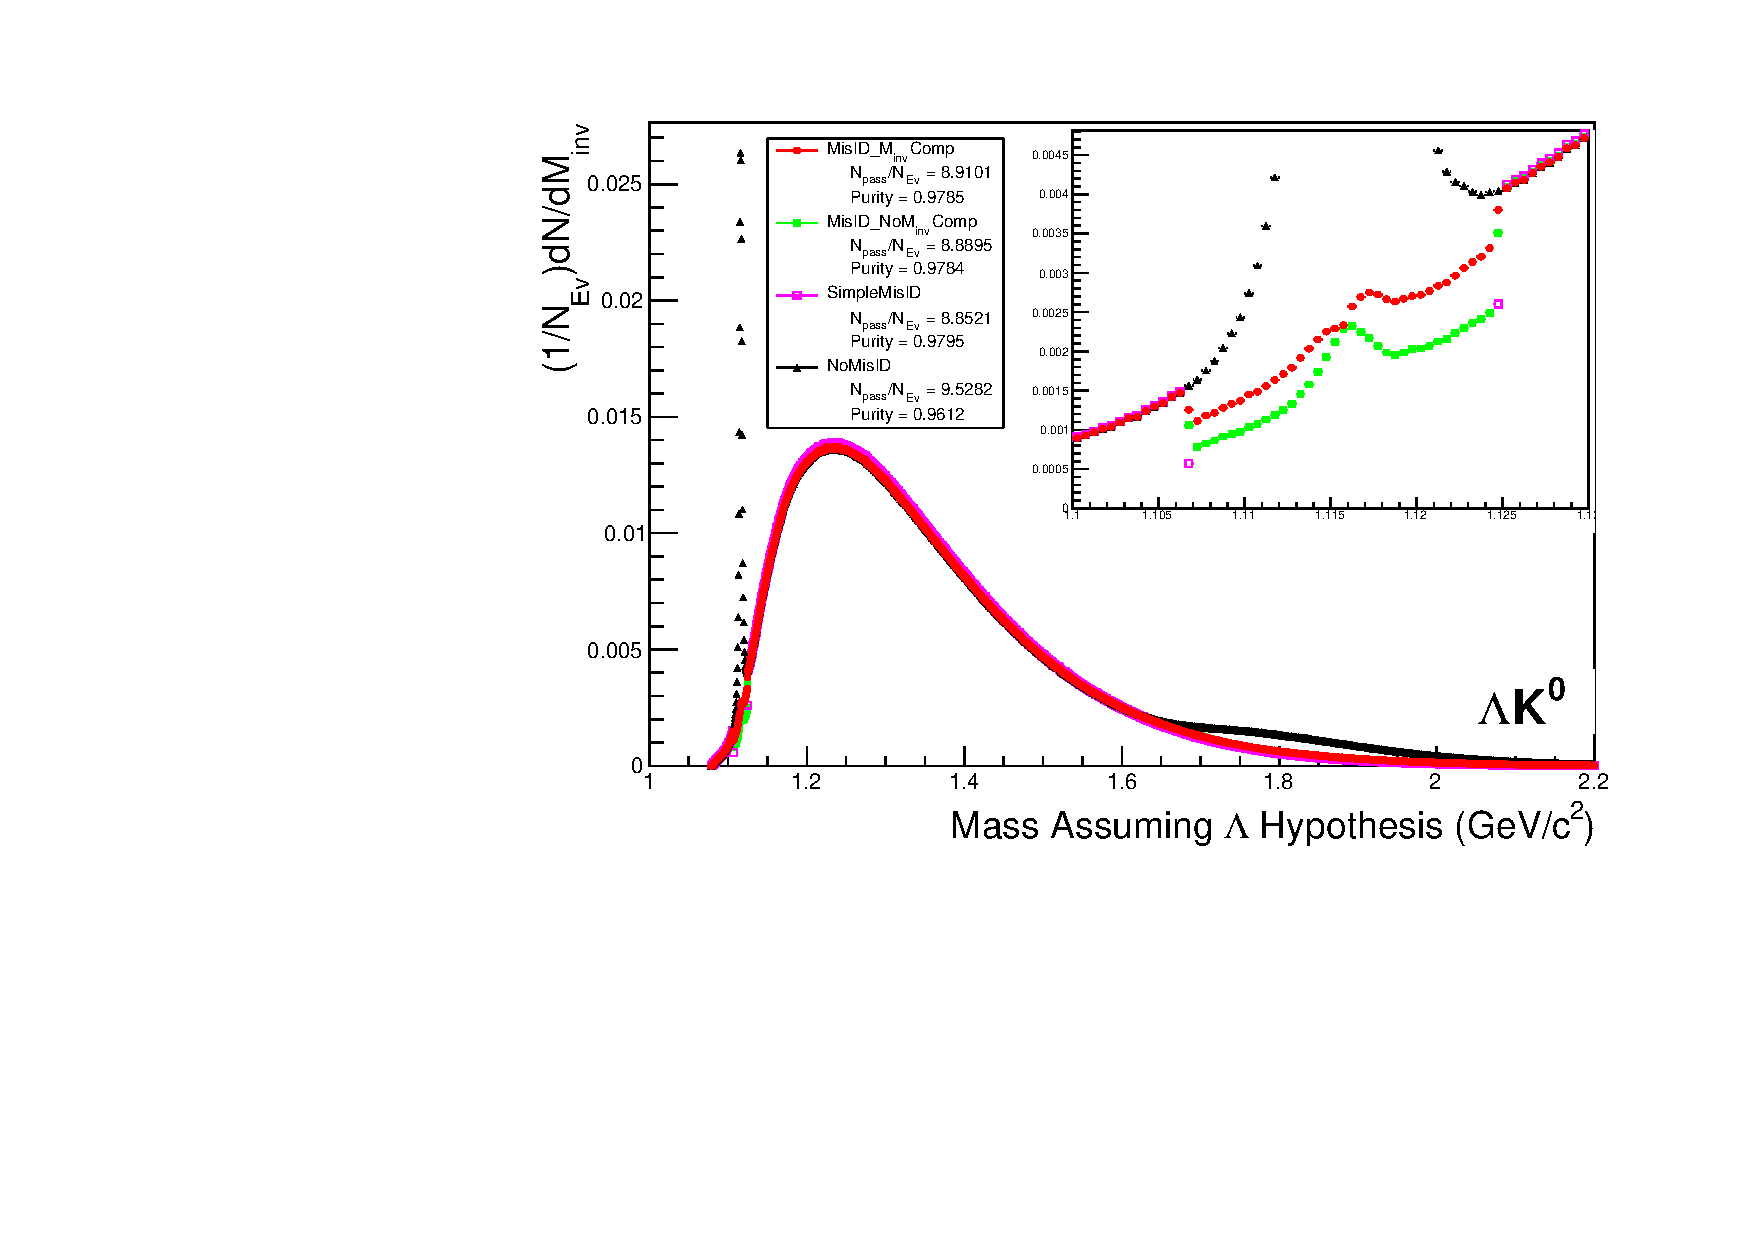
\includegraphics[width=0.5\textwidth]{3_DataSelection/Figures/MassAssHypotheses/canMassAssLamHypCompare_LamK0_wNoMisID.pdf}}
  %%----start of second subfigure---
  \subfloat[Mass assuming \ALam-hypothesis for \Ks collection, i.e. assume the daughters are $\pi^{+}\bar{p}^{-}$ instead of $\pi^{+}\pi^{-}$.]{
    \label{fig:MassAsscLamHyp:b}
    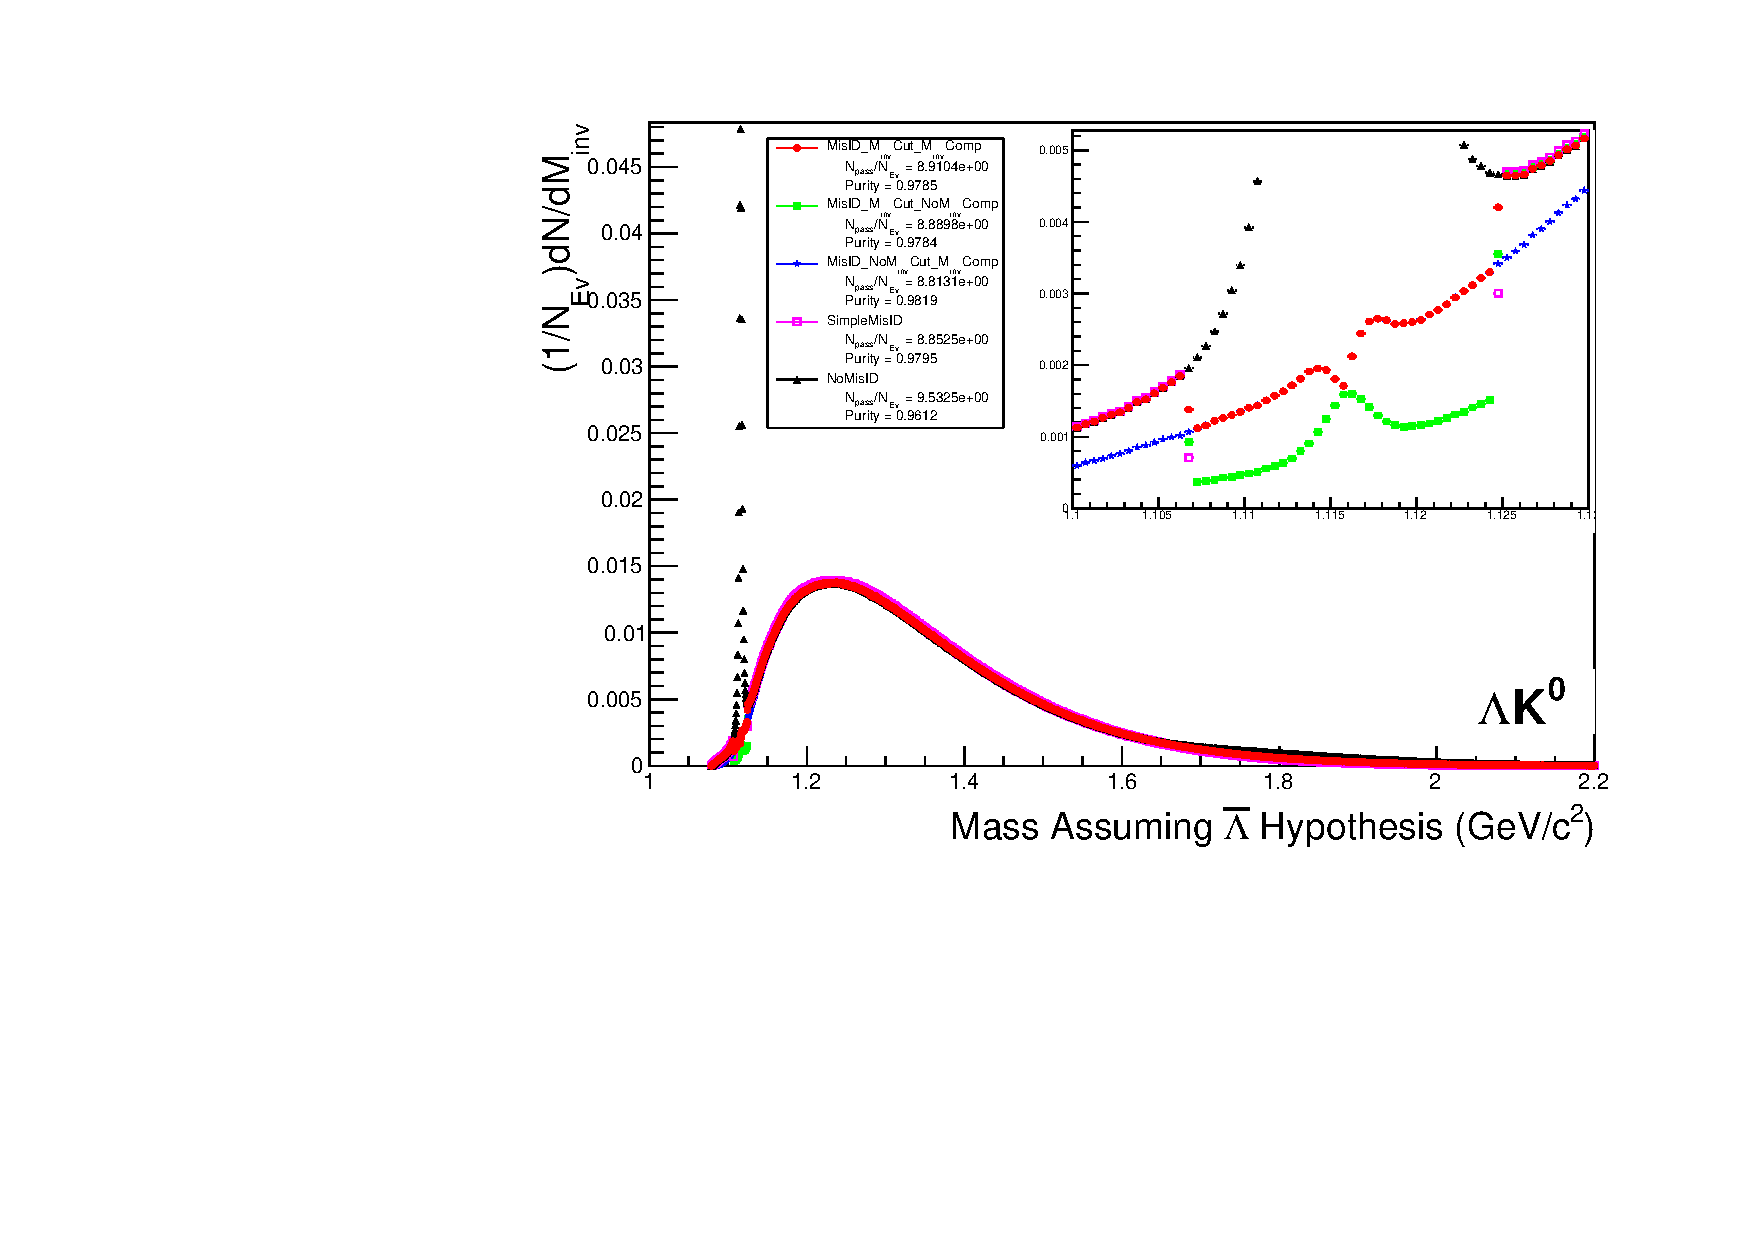
\includegraphics[width=0.5\textwidth]{3_DataSelection/Figures/MassAssHypotheses/canMassAssALamHypCompare_LamK0_wNoMisID.pdf}}
  %%----overall caption----
  \caption[\LamALam contamination in \Ks collection]{Mass assuming \Lam-hypothesis (\ref{fig:MassAsscLamHyp:a}) and \ALam-hypothesis (\ref{fig:MassAsscLamHyp:b}) for \Ks collection.
  The ``NoMisID" distribution (black triangles) uses the V0 finder without any attempt to remove misidentified \Lam and \ALam.
  The peak in the ``NoMisID" distribution around \minv = 1.115 GeV/$c^{2}$ contains misidentified \Lam (\ref{fig:MassAsscLamHyp:a}) and \ALam (\ref{fig:MassAsscLamHyp:b}) particles in our \Ks collection.  
  ``SimpleMisID" (pink squares) simply cuts out the entire peak, which throws away some good \Ks particles.
  ``MisID\_NoM$_{\mathrm{inv}}$Comp" (green squares) uses the misidentification cut outlined in the text, but does not utilize the final invariant mass comparison step.
  ``MisID\_M$_{\mathrm{inv}}$Comp" (red circles) utilizes the full misidentification methods, and is currently used for this analysis.
  ``N$_{\mathrm{pass}}$/N$_{\mathrm{ev}}$" is the total number of \Ks particles found, normalized by the total number of events.  The purity of the collection is also listed. 
  Also note, the relative excess of the ``NoMisID" distribution around 1.65 $<$ \minv $<$ 2.1 GeV/$c^{2}$ shows misidentified \ALam (\ref{fig:MassAsscLamHyp:a}) and \Lam (\ref{fig:MassAsscLamHyp:b}) particles in our \Ks collection.}
  \label{fig:MassAsscLamHyp}
\end{figure}



As can be seen in Figure \ref{fig:MassAsscLamHyp}, some misidentified \Lam and \ALam particles contaminate our \Ks sample.
Figure \ref{fig:MassAsscLamHyp:a} shows the mass assuming \Lam-hypothesis for the \Ks collection, i.e. assume the daughters are p$^{+}\pi^{-}$ instead of $\pi^{+}\pi^{-}$.
Figure \ref{fig:MassAsscLamHyp:b} is similar, but shows the mass assuming \ALam-hypothesis for the collection, i.e. assume the daughters are $\pi^{+}\bar{p}^{-}$ instead of $\pi^{+}\pi^{-}$.
The \Lam contamination can be seen in \ref{fig:MassAsscLamHyp:a}, and the \ALam contamination in \ref{fig:MassAsscLamHyp:b}, in the peaks around \minv = 1.115 GeV/$c^{2}$.
Additionally, the \ALam contamination is visible in Figure \ref{fig:MassAsscLamHyp:a}, and the \Lam contamination visible in Figure \ref{fig:MassAsscLamHyp:b}, in the region of excess around 1.65 $<$ \minv $<$ 2.1 GeV/$c^{2}$.
This is confirmed as the number of misidentified \Lam particles in the sharp peak of Figure \ref{fig:MassAsscLamHyp:a} (misidentified \ALam particles in the sharp peak of Figure \ref{fig:MassAsscLamHyp:b}) approximately equals the excess found in the 1.65 $<$ \minv $<$ 2.1 GeV/$c^{2}$ region of Figure \ref{fig:MassAsscLamHyp:a} (Figure \ref{fig:MassAsscLamHyp:b}).

The peaks around \minv = 1.115 GeV/$c^{2}$ in Figure \ref{fig:MassAsscLamHyp} contain both misidentified \LamALam particles and good \Ks.
If one simply cuts out the entire peak, some good \Ks particles will be lost.
Ideally, the \Ks selection and \LamALam misidentification cuts can be selected such that the peak is removed from this plot while leaving the underlying distribution continuous.
To attempt to remove these \Lam and \ALam contaminations without throwing away good \Ks particles, the misidentification cuts introduced in Sec. \ref{GenV0Reco} were imposed.

\end{document}